
\documentclass[11pt]{article} 

\usepackage[utf8]{inputenc} 
\usepackage{geometry} 
\usepackage{graphicx}% http://ctan.org/pkg/graphicx
\usepackage{array}% http://ctan.org/pkg/array
\usepackage{amsmath}
\usepackage{empheq}

\geometry{a4paper} 

\vspace{2cm}
\setlength{\parindent}{0cm}
\usepackage{graphicx,wrapfig,placeins}

\title{Disney BRDF}
\author{Chichi Francesco}

\begin{document}
\maketitle
\graphicspath{{img/}}
\section{Introduction}
	This project aims to implement the \textbf{Bidirectional Reflectance Distribution Function} developed by the Disney company. 

\newpage
\section{Bidirectional reflectance distribution function (BRDF)}
The bidirectional reflectance distribution function is a function $ f(x,i,o) $ that defines how light is reflected at an opaque surface (figure \ref{fig:reflect}), and is defined as the ratio of the differential reflected radiance over the
differential incident irradiance. 
In simple terms, the BRDF define the probability that a photon coming from a direction \textit{i} is reflected in a direction \textit{r}, after the collision with an opaque surface.
We can so define it as \cite{slide}:
\begin{align*}
	f(x,i,o)=\frac{\delta L_r(x,o)}{\delta E_i(x,i)} = \frac{\delta L_r(x,o)}{L_i(x,i)(n_x\cdot i) \delta \omega_i} 
\end{align*}

\begin{figure} [ht]
	\centering
	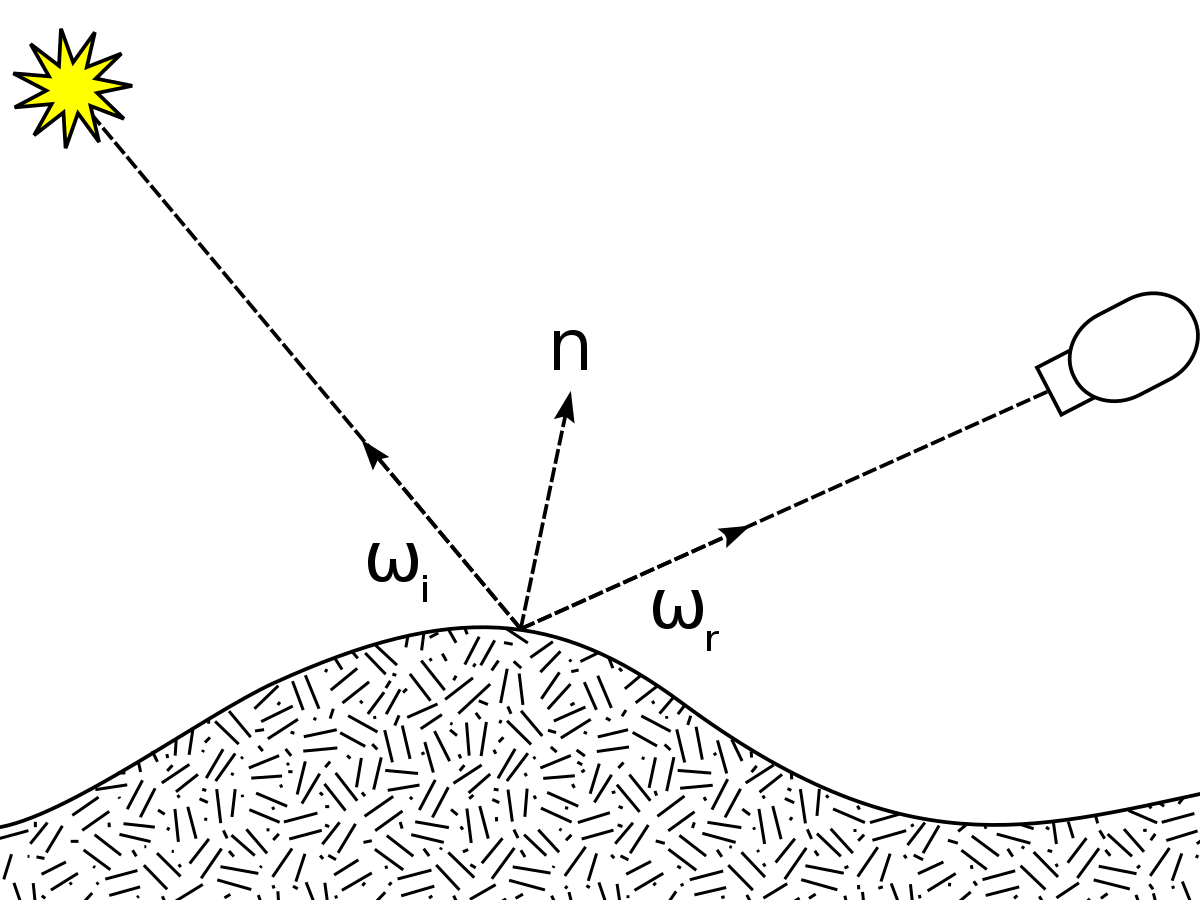
\includegraphics[width=0.5\linewidth]{img/reflect}
	\caption{A graphical example of the photon's reflection on an opaque surface.}
	\label{fig:reflect}
\end{figure}

A physically based specular BRDF is based on micro-facet theory, which describe a surface is composed of many micro-facets and each micro-facet will only reflect light in a single direction according to their normal(m) (figure \ref{fig:microfacet}) \cite{slide,microfacet} 

\begin{figure}[ht]
	\centering
	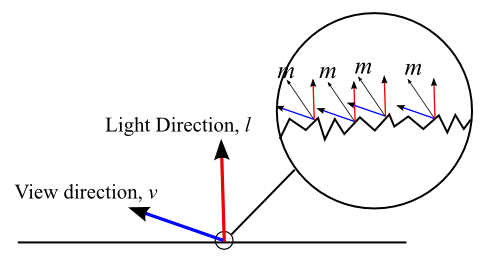
\includegraphics[width=0.5\linewidth]{img/microfacet}
	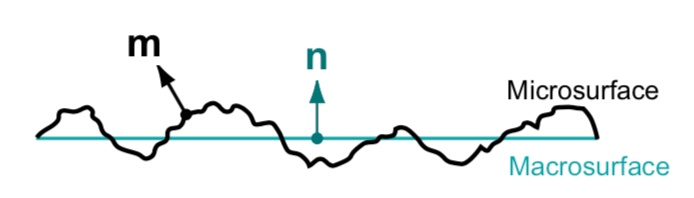
\includegraphics[width=0.5\linewidth]{img/microfacet2}
	\caption{A graphical example of the photon's reflection on the microfacets surfaces.}
	\label{fig:microfacet}
\end{figure}

So, the BRDF is essentially the "average" value of all these reflection events among all the micro-facets.
The microfacet reflection is then the normalized product of three terms:
\begin{align*}
	f_r(i,o)&=\frac{F(i,h)D(h)G(h,i,o)}{4|n\cdot i||n\cdot o|}\\
	h&= \frac{i+o}{|i+o|}
\end{align*}
Where F is the fresnel term, that take accounts for difference at grazing angle, the microfacet distribution D describes the statistical distribution of microfacets in a surface and the shadow-masking term G, that corrects for facets not visible from light or from the point of view (fig \ref{fig:visible})

\begin{figure}[ht]
	\centering
	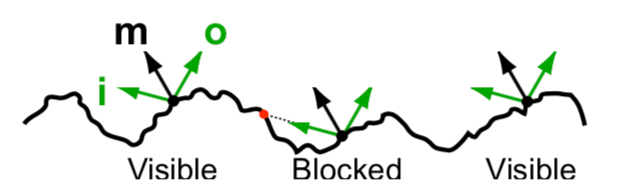
\includegraphics[width=0.5\linewidth]{img/visible}
	\caption{Example of the microfacet surface visibility.}
	\label{fig:visible}
\end{figure}


\section{Disney BRDF}
The Disney company studied and developed a custom BRDF, in order to increase the
richness of all of their materials while making lighting responses more consistent between materials and
environments and also wanted to improve artist productivity through the use of simplified controls.\\
They uses the Lambert diffuse model, which give a good physical representation of the scene, but reshaping the component of this equation.\\\\
Lambert model: 
\begin{align*}
 f(l,v) &= diffuse + \frac{D(\theta_h)F(\theta_d)G(\theta_l,\theta_v)}{4cos\theta_lcos\theta_v}\\
\end{align*}
Where $\theta_l$ and $\theta_v$ are the angles of incidence of the light and view vectors, \textit{l} and \textit{v}, with respect to the normal.
$\theta_h$ is the angle between the normal and the half-vector $h = \frac{l+v}{|l+v|} $, and $\theta_d$ is the "difference" angle between \textit{l} and \textit{h}, or symmetricallly between \textit{v} and \textit{h}.

\subsection{Diffuse model}
Diffuse reflectance represents light that is refracted into the surface, scattered, partially absorbed,
and re-emitted. Given that some of the light is absorbed, the diffuse response will be tinted with the
surface color, and any portion of a non-metallic material that is tinted can be considered to be diffuse.\\\\
The problem, for the Disney company, was that this model is often too dark on the edges, and adding a Fresnel factor to make it more physically plausible only makes it darker.\\
The model developed aims to increase the refraction at gazing angles, the angle between the tangent to the surface and the outgoing ray, when the light enters and exits the sides of micro-facet surfaces.

The modified diffuse model is the following:\\\\
\begin{align*}
 \frac{baseColor}{\pi} (1 + (F_{D90} - 1)(1 - cos\theta_l)^5)(1 + (F_{D90} -1)(1 - cos\theta_v)^5)\\\\
\end{align*}
where  $F_{D90} = 0.5 + 2cos\theta_d^2$ \textit{roughness}\\\\


The resulting model have a redocted incident diffuse reflectance by 0.5 at gazing angles for smooth surfaces and an increased response by up to 2.5 for the rough ones.
\subsection{Specular D}
The most popular models is the GGX, wich is equivalent to the Trowbridge-Reitz (1975) one ($D_{TR}$). 
However, this distribution still does not have a long enough tail for many materials.
One of the other distributions, from Berry (1923), has a very similar
form but with an exponent of 1 instead of 2 resulting in an even longer tail. This suggests a more general
distribution with a variable exponent, introduced here and dubbed Generalized-Trowbridge-Reitz, or
GTR:
\begin{align*}
  D_{Berry} &= c/(\alpha^2 cos^2\theta_h + sin^2\theta_h) \\
  D_{TR} &= c/(\alpha^2 cos^2\theta_h + sin^2\theta_h)^2 \\
  D_{GTR} &= c/(\alpha^2 cos^2\theta_h + sin^2\theta_h)^\gamma
\end{align*}
 In each of these distributions, $\textit{c}$ is a scaling constant, $\alpha$ is a roughness parameter with values between 0 (a perfectly smooth distribution) and in 1 (a perfectly rough).\\
The $\gamma$ value have 2 fixet value: $\gamma = 2$ for the metallic material and $\gamma = 1$ for the non-metallic one.\\
For roughness, the $\alpha$ was remapped to the $roughness^2$, in order to achieve more intuitive value to represent shiny materials.

\subsection{Specular F}
In graphics, one of the most diffuse model for represent the Fresnel reflection $ (k_r) $ and transmission $ (k_t = 1 - k_r) $ is the Schlick's approximation:
\begin{align*}
	k_r = k_s^0 + (1 - k_s^0)(1 - cos\theta_d)^5
\end{align*}
Where $k_s^0$ represents the specular reflectance at nominal incidance.
This approximated model has not been changed by Disney.
\subsection{Specular G}
For the G component, is used a GGX, with only one difference: in order to reduce the
extreme gain for shiny surfaces, the $\alpha_g$ value was linearly scaled from the [0,1] range to a reduced one, [0.5,1].
So, the new value becomes:
\begin{align*}
	\alpha_g = (0.5 + roughness/2)^2
\end{align*}
\subsection{Yocto-GL Implementation}
The Yocto-GL is implemented as a two file library: \textit{yocto\_gl.h} and \textit{yocto\_gl.cpp}.
This project has been developed as an extension of this library with the addition of the disney path tracer.\\
In order to preserve the user interface provided by this library, two application concerning the path tracing, \textit{ytrace.cpp} and \textit{yitrace.cpp}, have been modified, so that the user can choose to use the path tracer using the disney BRDF only changin the shader parameter to \textit{path\_disney}.\\
Other two parameters were added, respectively the \textit{d\_gamma} and the \textit{d\_constant}, in order to easily manipulate this value for the specular D component.

\begin{table}[ht]
  \centering
  \begin{tabular}{ | c | c |}
    \hline
    normal & const 0.005 gamma 1 \\ \hline
    \begin{minipage}{.455\textwidth}
      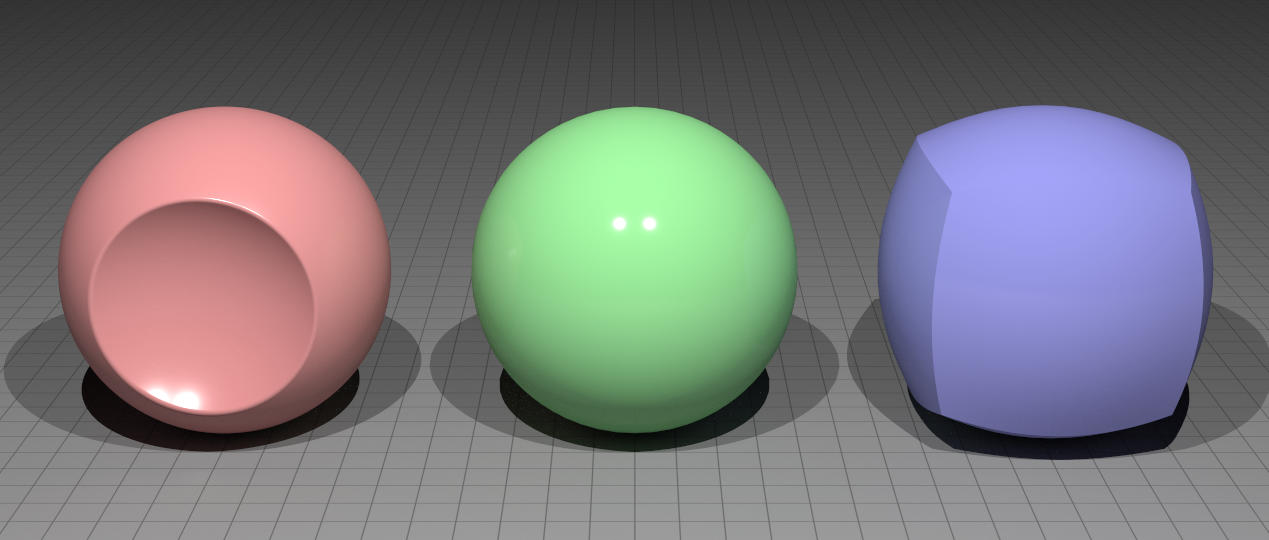
\includegraphics[scale=0.15]{img/obj/basic_pl/basic_pl.jpg}
    \end{minipage}
    &
    \begin{minipage}{.455\textwidth}
      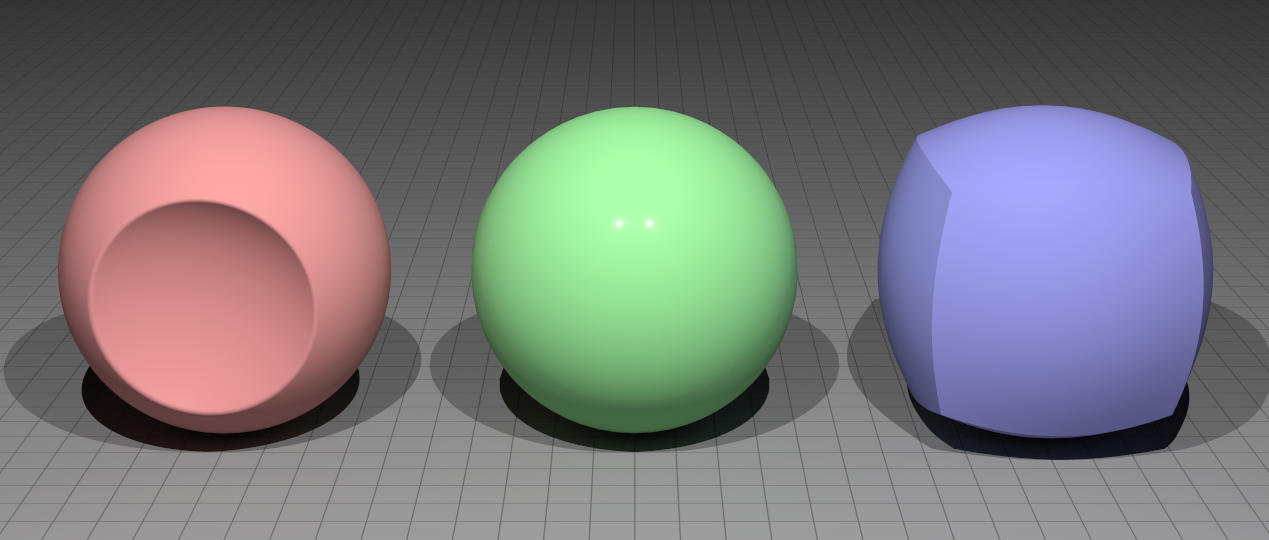
\includegraphics[scale=0.15]{img/obj/basic_pl/basic_pl_disney_dg1_dc005.jpg}
    \end{minipage}
    \\ \hline
  \end{tabular}\\
  \begin{tabular}{ | c | c |}
    \hline
    const 0.03 gamma 1 & const 0.005 gamma 2 \\ \hline
    \begin{minipage}{.455\textwidth}
      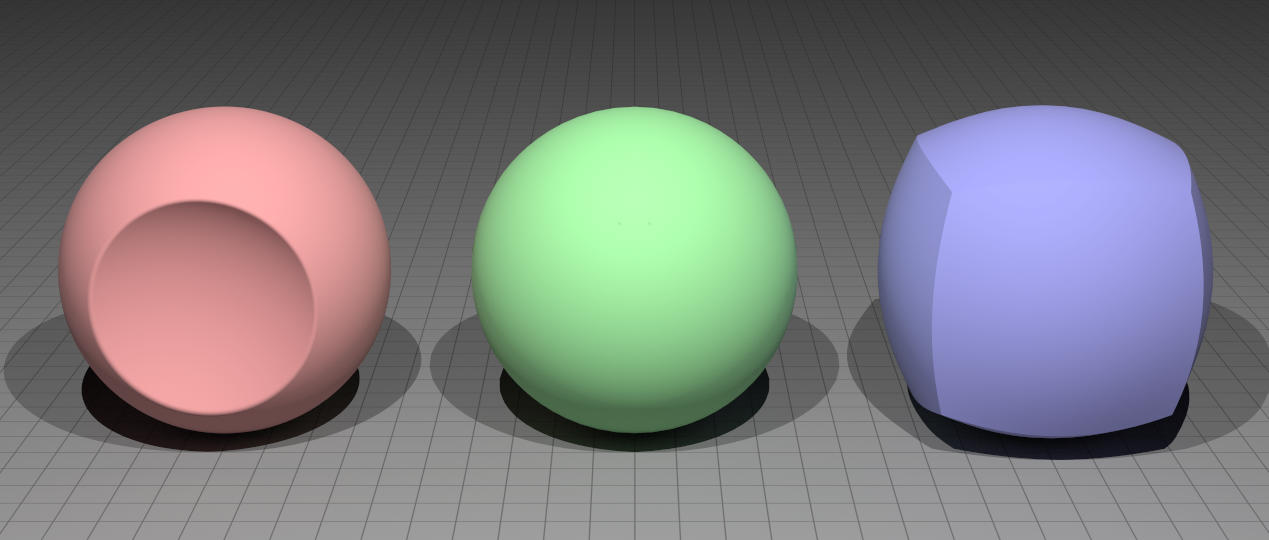
\includegraphics[scale=0.15]{img/obj/basic_pl/basic_pl_disney_dc03_dg1.jpg}
    \end{minipage}
    &
    \begin{minipage}{.455\textwidth}
      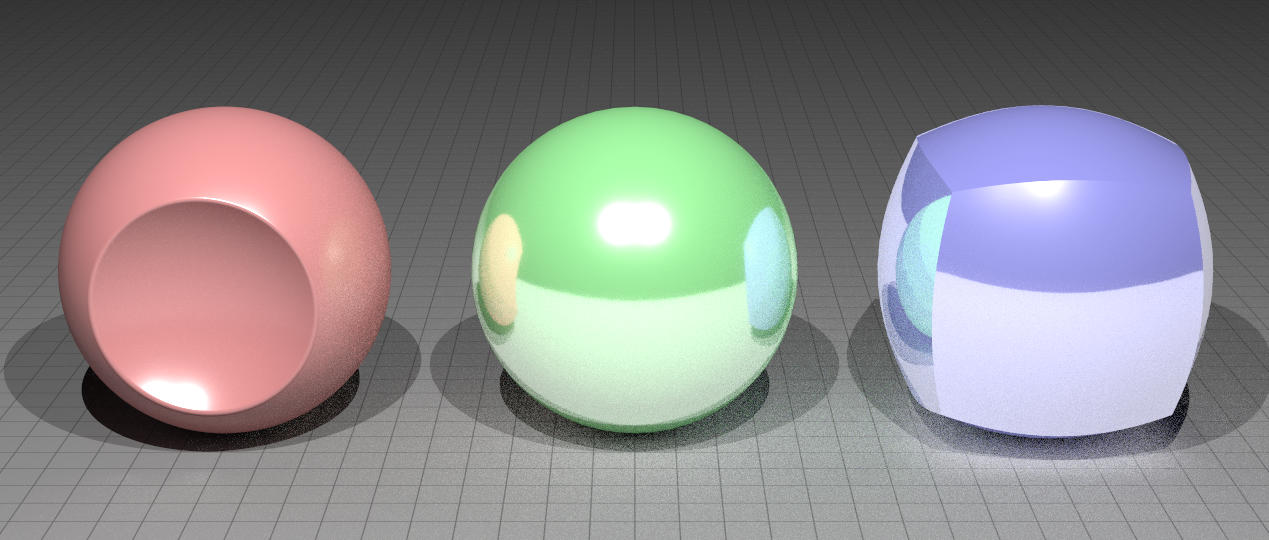
\includegraphics[scale=0.15]{img/obj/basic_pl/basic_pl_disney_dc005_dg2.jpg}
    \end{minipage}
    \\ \hline
  \end{tabular}
   \caption{\textit{basic\_pl} object rendered with the basic path tracer and with the one of Disney}\label{tbl:myLboro}
\end{table}



\section{Conclusions}


\section{Other libraries}
\begin{itemize}
	\item \textbf{yocto-gl:}
		Yocto/GL is a collection utilities for building physically-based graphics algorithms implemented as a two-file library, and released under the MIT license.
		
\end{itemize}

\begin{thebibliography}{9}
	\bibitem{disney} 
	Brent Burley, Walt Disney Animation Studios. 
	\textit{Physically-Based Shading at Disney}.
	
	\bibitem{slide} 
	Fabio Pellacini's slide. 
	\textit{http://pellacini.di.uniroma1.it/teaching/graphics17b/index.html}

	\bibitem{microfacet} 
	Microfacet BRDF. 
	\textit{http://simonstechblog.blogspot.it/2011/12/microfacet-brdf.html}
	
	
	
\end{thebibliography}


\end{document}
